\documentclass[a4paper, 12pt]{article}
\usepackage[russian]{babel}
\usepackage[T2A]{fontenc}
\usepackage[utf8]{inputenc}


\usepackage{xcolor}

\usepackage{hyperref}
\definecolor{linkcolor}{HTML}{44D663} % цвет ссылок
\definecolor{urlcolor}{HTML}{031A9B} % цвет гиперссылок

\hypersetup{pdfstartview=FitH,  linkcolor=black,urlcolor=urlcolor, colorlinks=true}

\usepackage{graphicx}

\usepackage{multirow}
\usepackage{multicol}

\usepackage{amsmath} 
\usepackage{listings}
\usepackage{xcolor}
\usepackage{color}
\usepackage{amsmath}

\definecolor{dkgreen}{rgb}{0,0.6,0}
\definecolor{gray}{rgb}{0.5,0.5,0.5}
\definecolor{mauve}{rgb}{0.58,0,0.82}
\lstset { %
	language=C++,
	backgroundcolor=\color{black!5}, % set backgroundcolor
	basicstyle=\footnotesize,% basic font setting
	tabsize=3,
	breaklines=true,
	breakatwhitespace=true,
	numbers=left,
	% Стиль литералов
}

\usepackage{pgfplots}
\pgfplotsset{compat=1.9}



\usepackage{amsmath}

\usepackage{amsmath, amsfonts}



\begin{document}
	\newpage
	
	\begin{figure}[h] % [h] означает, что рисунок будет размещен здесь, а не автоматически в конце раздела или страницы
		\centering % Выравнивание по центру
		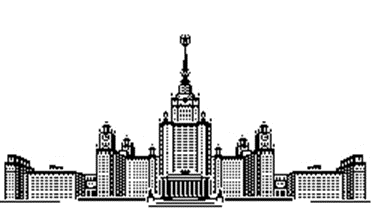
\includegraphics[width=0.5\textwidth]{МГУ.PNG} % Вставка изображения. Укажите путь к вашему изображению вместо example-image
		% Подпись к рисунку
		
	\end{figure}
	
	\begin{center}
		\text{\large{Московский государственный университет имени М.В.Ломоносова}} \\
		
		\text{\large{Факультет вычислительной математики и кибернетики}} \\
		
		\text{\large{Кафедра математической физики}} 
		
		
	\end{center}
	
	
	
	\vspace{5em}
	
	\begin{center}
		\textbf{\LARGE{Численный метод вычисления электромагнитного поля электрического диполя
				в плоскослоистой среде со слоем графена}}
	\end{center}
	
	\vspace{2em}
	
	\begin{center}
		\large{Преддипломная работа студента 4-го курса Артемова Арсения}
	\end{center}
	
	\vspace{6em}
	
	\begin{flushright}
		
		\large{	Научный руководитель \linebreak
			к.ф.-м.н. Березина Н. И.}\\
		\vspace{3em}
		
		
	\end{flushright}
	
	\vspace{2em}
	
	\vspace{\fill}
	
	\begin{center}
		\textbf{{\large Москва 2024}}
	\end{center}
	\thispagestyle{empty} 
	
	
	\tableofcontents
	
	\newpage
	
	\section{Введение} 
	
	Графен - двумерный кристалл углерода, полученный в 2004 году британскими учёными российского происхождения Андреем Геймом и Константином Новоселовым из Манчестерского университета, представляет собой один из самых интригующих материалов в современной науке и технологиях. Его уникальные физические и химические свойства, такие как высокая прочность, высокая электропроводность, большая удельная поверхность и прозрачность, делают его перспективным объектом исследования в различных областях, включая электронику, оптику, энергетику и биомедицину.
	
	Графен обладает рядом фундаментальных свойств, которые делают его уникальным материалом. Его структура представляет собой плоскую, атомарно тонкую сетку углеродных атомов, организованных в гексагональную решетку, подобную пчелиному соту. Благодаря этой уникальной структуре графен обладает экстремальными механическими, электронными и оптическими свойствами.
	
	Важно отметить, что графен является не только объектом активного экспериментального исследования, но и предметом интенсивных теоретических исследований. Множество работ посвящены изучению электронных структур, фазовых переходов, электропроводности и других аспектов его поведения.
	
	Одним из наиболее важных аспектов исследования графена является его влияние на электромагнитные явления в окружающей среде. В частности, изучение взаимодействия графена с электромагнитными полями открывает новые перспективы для создания сенсоров, устройств связи и оптических систем с улучшенными характеристиками.
	
	В данной работе мы сосредоточимся на изучении электромагнитного поля диполя в плоскослоистой среде, содержащей графеновый слой. Анализ взаимодействия диполя с графеном позволит нам лучше понять влияние этого уникального материала на электромагнитные процессы.
	
	\newpage
	
	\section{Электромагнитное поле диполя в плоскослоистой среде с графеновым  слоем}
	
	\subsection{Постановка задачи}
	
	Дана плоскослоистая среда состоящая из 2х слоев с различными проводимостями $$\varepsilon_1, \varepsilon_2 - const, $$разделенных слоем графена. 
	В точке $M_s(0,0,z_s) $ находится источник электромагнитного поля - электрический диполь, его поле изменяется во времени по закону $e^{-i\omega t}$.
	
	\begin{figure}[h] % [h] означает, что рисунок будет размещен здесь, а не автоматически в конце раздела или страницы
		\centering % Выравнивание по центру
		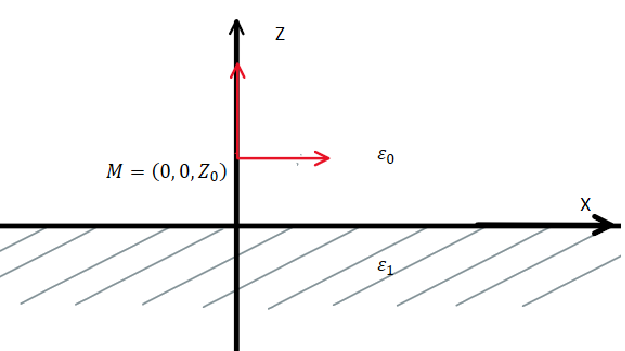
\includegraphics[width=0.5\textwidth]{Рис 6.PNG} % Вставка изображения. Укажите путь к вашему изображению вместо example-image
		\caption{Плоскослоистая среда с графеновым слоем} % Подпись к рисунку
		\label{fig:example6} % Метка для ссылки на рисунок
	\end{figure}
	
	Тогда система уравнений Максвелла имеет вид:
	
	
	\begin{equation}
		\begin{cases} rot \vec{H} = -i \omega \varepsilon \vec{E} + j_{ст} \\ rot \vec{E} = iw\mu \vec{H} \end{cases}
	\end{equation}
	
	На обеих границах выполняются условия непрерывности касательных компонент полей-
	
	\begin{equation}
		\begin{cases}
			[\vec{n} \times \vec{E} ]_S = 0, \\
			[\vec{n} \times \vec{H}]_S = \delta E_{\tau} 
		\end{cases}
	\end{equation}
	
	где $\delta = \delta_1 + \delta_2 * {|E_{\tau}|}^2$, где $\delta_2 \approx 0$.
	
	
	Введем 2 векторных потенциала - $A$ и $a$ с калибровками Лоренца:
	
	$$\begin{cases}
		\vec{E} = \vec{E^{*}} + \vec{E^{**}} \\
		\vec{E} = \vec{H^{*}} + \vec{H^{**}}
	\end{cases}$$
	
	\begin{equation}
		\begin{cases}
			\vec{H^*_{1, 2}} = \frac{k^2_{1, 2}a}{\mu_0} + \frac{grad div \vec{a}}{\mu_0}  \\
			\vec{E^*_{1, 2}} = i \omega rot \vec{a}
		\end{cases}
	\end{equation}
	
	\begin{equation}
		\begin{cases}
			\vec{H^{**}_{1, 2}} = \frac{rot \vec{A}}{\mu_0} \\
			\vec{E^{**}_{1, 2}} = i \omega \vec{A} + grad(\frac{i \omega}{k^2_{1, 2}} div \vec{A}) \\
		\end{cases}
	\end{equation}
	
	Граничные условия (47) можно переписать в виде:
	
	\begin{equation*}
		\tag{2.1}
		\begin{cases}
			[E_x] = 0 \\
			[E_y] = 0 \\
			[H_x] = \delta E_{x_1} \\
			[H_y] = \delta E_{y_1}
			
		\end{cases}
	\end{equation*}
	
	\subsection{Вертикальный диполь}
	
	Подставив (48, 49) в (47.1) получим в $z = 0$:
	
	\begin{equation}
		\begin{cases}
			\frac{1}{k_1^2} \frac{\partial A_{z_1}}{\partial z} = \frac{1}{k_2^2} \frac{\partial A_{z_2}}{\partial z} \\
			
			a_{z_1} = a_{z_2} \\
			
			-\frac{\partial A_{z_2}}{\partial x} + \frac{\partial^2 a_{z_2}}{\partial y \partial z} + \frac{\partial A_{z_1}}{\partial x} - \frac{\partial^2 a_{z_1}}{\partial y \partial z} = i \omega \delta (\frac{1}{k_1^2} \frac{\partial^2 A_{z_1}}{\partial y \partial z} - \frac{\partial a_{z_1}}{\partial x}) \\
			
			\frac{\partial A_{z_2}}{\partial y} + \frac{\partial^2 a_{z_2}}{\partial x \partial z} - \frac{\partial A_{z_1}}{\partial y} - \frac{\partial^2 a_{z_1}}{\partial x \partial z} = i \omega \delta (\frac{1}{k_1^2} \frac{\partial^2 A_{z_1}}{\partial x \partial z} + \frac{\partial a_{z_1}}{\partial y})
			
			
		\end{cases}
	\end{equation}
	
	
	так как 
	
	\begin{equation}
		\begin{aligned}
			H_x = \frac{1}{\mu_0} (\frac{\partial ^ 2 a_z}{\partial x \partial z} + \frac{\partial A_z}{\partial y}) \\
			H_y = \frac{1}{\mu_0} (\frac{\partial ^ 2 a_z}{\partial y \partial z} - \frac{\partial A_z}{\partial x}) \\
			E_x = i \omega \delta (\frac{1}{k_1^2} \frac{\partial^2 A_{z_1}}{\partial y \partial z} - \frac{\partial a_{z_1}}{\partial x}) \\			
			E_y = i \omega \delta (\frac{1}{k_1^2} \frac{\partial^2 A_{z_1}}{\partial x \partial z} + \frac{\partial a_{z_1}}{\partial y})
		\end{aligned}
	\end{equation}
	
	при $z \neq z_0$ $A_z$ и $a_z$ удовлетворяют 
	
	\begin{equation}
		\begin{aligned}
			\Delta A_z + k^2 A_z = 0 \\
			\Delta a_z + k^2 a_z = 0
		\end{aligned}
	\end{equation}
	
	при приближении к источнику должно выполняться:
	
	\begin{equation}
		A_z \rightarrow \frac{M}{4 \pi} \frac{\exp{i k_1 R}}{R} 
	\end{equation}
	
	где, $R = \sqrt{x^2 + y^2 + {(z - z_0)} ^ 2}$.
	
	при $R \rightarrow \infty$ выполняются
	
	\begin{equation}
		\begin{cases}
			A_z = O_{R \rightarrow \infty}(\frac{1}{R}) \\
			\frac{\partial A_z}{\partial R} + i A_z k = o_{R \rightarrow \infty}(\frac{1}{R})
		\end{cases}
	\end{equation}
	
	Будем искать решение в виде преобразований Ханкеля (аналогично случаю без графена)
	
	\begin{equation}
		\begin{aligned}
			a_z = \frac{I \mu_0 }{4 \pi} \int_0^{\infty} X J_0(mz)dm \\
			A_z = \frac{I \mu_0 }{4 \pi} \int_0^{\infty} V J_0(mz)dm
		\end{aligned}
	\end{equation}
	
	тогда $X$ и $V$ удовлетворяют
	
	\begin{equation}
		\begin{aligned}
			\frac{\partial^2 X}{\partial z^2} - n_{1, 2}^2 X = 0 \\
			\frac{\partial^2 V}{\partial z^2} - n_{1, 2}^2 V = 0 \\
		\end{aligned}
	\end{equation}
	
	где $n_{1, 2}^2 = m^2 - k_{1, 2}^2$, $Re (n) > 0$
	
	\begin{equation*}
		\tag{50.1}
		\begin{aligned}
			& \frac{1}{k_1^2} \frac{\partial A_{z_1}}{\partial z} = \frac{1}{k_1^2} \frac{\partial A_{z_2}}{\partial z} \\
			&a_{z_1} = a_{z_2} \\
			& A_{z_2} - A_{z_1} = i \omega \delta a_{z_1} \\
			&\frac{\partial a_{z_2}}{\partial z} - \frac{\partial a_{z_1}}{\partial z} = -i \omega \delta \frac{1}{k_1^2} \frac{\partial A_{z_1}}{\partial z} \\ 
		\end{aligned}
	\end{equation*}
	
	для $X$ и $V$ получим в $z = 0$:
	
	\begin{equation}
		\begin{aligned}
			& \frac{1}{k_1^2} \frac{\partial V_1}{\partial z} = \frac{1}{k_1^2} \frac{\partial V_2}{\partial z} \\
			&X_1 = X_2 \\
			& V_2 - V_1 = i \omega \delta X_2 \\
			&\frac{\partial X_2}{\partial z} - \frac{\partial X_1}{\partial z} = -i \omega \delta \frac{1}{k_2^2} \frac{\partial V_2}{\partial z} \\ 
		\end{aligned}
	\end{equation}
	\newpage
	в $z = z_0$
	
	
	\begin{equation}
		\begin{aligned}
			&\frac{\partial X_1^*}{\partial z} = \frac{\partial X_1}{\partial z} \\
			&X_1^* = X_1 \\
			&\frac{\partial V_1^*}{\partial z} - \frac{\partial V_1}{\partial z} = 2 \\
			&V_1^* = V_1 \\
		\end{aligned}
	\end{equation}
	
	Будем искать $V_1, V_2, V_1^*, X_1, X_2$ в виде:
	
	\begin{equation}
		\begin{aligned}
			&V: \\
			& z > z_0 \space 	&V_1^* = \beta_1^* e^{-n_1z} \\
			& z_0 > z > 0 \space	 &V_1 = \beta_1 e^{-n_1z} + \gamma_1 e^{n_1z} \\
			& z < 0 \space	&V_2 =  \gamma_2 e^{n_2z} \\
			&X: \\
			& z > 0 \space	&X_1 = d_1 e^{-n_1z} \\
			& z < 0	\space	&X_2 = c_2 e^{n_2z} 
		\end{aligned}
	\end{equation}
	
	Имеем 6 уравнений и 6 коэффициентов - решаем:
	
	\begin{equation}
		\begin{aligned}
			&\gamma_1 = \frac{e^{-n_1z_0}}{n_1} \\
			&\beta_1^* = \beta_1 - \frac{e^{n_z0}}{n_1} \\
			&L = -\frac{n_1 k_2^2}{n_2 k_1^2} + \frac{D^2 n_1}{(n_1 + n_2)k_1^2} \\
			&\beta_1 = \frac{e^{-n_1 z_0}}{n_1} (-1 + \frac{2L}{1 + L}) \\
			&\gamma_2 = \frac{k_2^2}{k_1^2} \frac{e^{-n_1z_0}}{n_2}(2 - \frac{D^2 n_1}{(n_1 + n_2)k_1^2}) \\
			&d_1 = c_1 = \frac{D e^{-n_1 z_0}}{(n_1 + n_2) k_1^2}(2 - \frac{D^2 n_1}{(n_1 + n_2)k_1^2}) \\ 
		\end{aligned}
	\end{equation}
	
	\newpage
	
	\subsection{Горизонтальный диполь}
	
	Для горизонтального диполя получим шраничные условия при $z = 0$:
	
	\begin{equation}
		\begin{cases}
			A_{x_1} = A_{x_2} \\
			A_{y_1} = A_{y_2} \\
			\frac{\partial A_{x_2}}{\partial z} - \frac{\partial A_{x_1}}{\partial z} = i \omega \delta A_{y_1} \\
			\frac{\partial A_{y_2}}{ \partial z} - \frac{\partial A_{y_1}}{\partial z} = i \omega \delta A_{x_1} \\
			a_{z_1} = a_{z_2} \\
			\frac{div(\vec{A_1})}{k_1^2} = \frac{div(\vec{A_2})}{k_2^2} \\
			A_{z_2} - A_{z_1} = i \omega \delta a_{z_1} \\
			\frac{\partial a_{z_2}}{\partial z} - \frac{\partial a_{z_1}}{\partial z} = i \omega \delta \frac{div(\vec{A_1})}{k_1^2}
		\end{cases}
	\end{equation}
	
	Так же вблизи источника выполняется:
	\begin{equation}
		A_x \rightarrow \frac{I \mu_0}{4 \pi} \frac{e^{i k_1 R}}{R}
	\end{equation}
	
	Представим $A_z$ и $a_z$ в виде:
	\begin{equation}
		\begin{aligned}
			A_z = \frac{\partial \text{П}}{\partial x} + \frac{\partial T}{\partial y} \\
			a_z = \frac{\partial P}{\partial x} + \frac{\partial Q}{\partial y} \\
		\end{aligned}
	\end{equation}
	
	тогда последние 2 условия из 61 можно переписать в виде:
	
	\begin{equation}
		\begin{aligned}
			&\frac{\partial \text{П}_2}{\partial x} - \frac{\partial \text{П}_1}{\partial x} + \frac{\partial T_2}{\partial y} - \frac{\partial T_1}{\partial y} = i \omega \delta (\frac{\partial P_1}{\partial x} + \frac{\partial Q_1}{\partial y}) \\
			&\frac{\partial^2 P_2}{\partial x \partial z} - \frac{\partial^2 P_1}{\partial x \partial z} + \frac{\partial^2 Q_2}{\partial y \partial z} - \frac{\partial^2 Q_1}{\partial y \partial z} = \frac{i \omega \delta}{k_1^2} (\frac{\partial A_{x_1}}{\partial x} + \frac{\partial A_{y_1}}{\partial y} + \frac{\partial^2 \textit{П}_1}{\partial x \partial z} + \frac{\partial ^ 2 T_1}{\partial y \partial z} )
		\end{aligned}
	\end{equation} 
	
	Для выполнения (64) достаточно системы:
	
	\begin{equation}
		\begin{cases}
			\text{П}_2 - \text{П}_1 = i \omega \delta P_1 \\
			\frac{\partial P_2}{\partial z} - \frac{\partial P_1}{\partial z} = \frac{i \omega \delta}{k_1^2} (A_{x_1} + \frac{\partial \text{П}_1}{\partial z}) \\
			T_2 - T_1 = i \omega \delta Q_1 \\
			\frac{\partial Q_2}{\partial z} - \frac{\partial Q_1}{\partial z} = \frac{i \omega \delta}{k_1^2} (A_{y_1} + \frac{\partial T_1}{\partial z}) \\
		\end{cases}
	\end{equation}
	
	\newpage
	
	так как:
	
	\begin{equation*}
		\begin{aligned}
			&a_{z_1} = a_{z_2} \\ 
			&\frac{div(\vec{A_1})}{k_1^2} = \frac{div(\vec{A_2})}{k_2^2} \\
		\end{aligned}
	\end{equation*}
	
	получаем 
	\begin{equation}
		
		\begin{cases}
			P_1 = P_2 \\
			\frac{1}{k_1^2}(A_{x_1} + \frac{\partial \text{П}_1}{\partial z}) = \frac{1}{k_2^2}(A_{x_2} + \frac{\partial \text{П}_2}{\partial z}) \\
			Q_1 = Q_2 \\
			\frac{1}{k_1^2}(A_{y_1} + \frac{\partial T_1}{\partial z}) = \frac{1}{k_2^2}(A_{y_2} + \frac{\partial T_2}{\partial z})
		\end{cases}
	\end{equation}
	
	Систему из 8 уравнений можно разбить на две независмые системы сожержащие $P, \text{П}, A_x$ и $T, Q, A_y$
	так же отдельно можем вычислить $A_x$ и $A_y$ из 61 и 62.
	
	Рассмотрим систему:
	
	\begin{equation}
		\begin{cases}
			P_1 = P_2 \\
			\frac{1}{k_1^2}(A_{x_1} + \frac{\partial \text{П}_1}{\partial z}) = \frac{1}{k_2^2}(A_{x_2} + \frac{\partial \text{П}_2}{\partial z}) \\
			\text{П}_2 - \text{П}_1 = i \omega \delta P_1 \\
			\frac{\partial P_2}{\partial z} - \frac{\partial P_1}{\partial z} = \frac{i \omega \delta}{k_1^2} (A_{x_1} + \frac{\partial \text{П}_1}{\partial z}) \\
		\end{cases}
	\end{equation}
	
	Будем искать $P, A_x, \text{П}$ в виде преобразований Ханкеля
	
	\begin{equation}
		\begin{aligned}
			& \text{П} = \frac{I \mu_0}{4 \pi} \int_0^{\infty} M J_0(mz) dm \\
			& P = \frac{I \mu_0}{4 \pi} \int_0^{\infty} N J_0(mz) dm \\
			& A_x = \frac{I \mu_0}{4 \pi} \int_0^{\infty} L J_0(mz) dm \\
			& A_y = \frac{I \mu_0}{4 \pi} \int_0^{\infty} S J_0(mz) dm \\
			& Q = \frac{I \mu_0}{4 \pi} \int_0^{\infty} K J_0(mz) dm \\
			& T = \frac{I \mu_0}{4 \pi} \int_0^{\infty} D J_0(mz) dm \\
		\end{aligned}
	\end{equation} 
	
	тогда систему, полученную из замены и уравнений Масвела:
	
	\begin{equation}
		\begin{cases}
			\Delta A_x + k^2 A_x = 0 \\
			\Delta A_y + k^2 A_y = 0 \\
			\Delta A_z + k^2 A_z = 0 \\
			\Delta a_z + k^2 a_z = 0 \\
		\end{cases}
	\end{equation}
	
	можно заменить достаточной:
	
	\begin{equation}
		\begin{cases}
			\frac{\partial \Delta M}{\partial x} + n^2 \frac{\partial M}{\partial x} = 0 \\
			\frac{\partial \Delta N}{\partial x} + n^2 \frac{\partial N}{\partial x} = 0 \\
			\frac{\partial \Delta K}{\partial y} + n^2 \frac{\partial K}{\partial y} = 0 \\
			\frac{\partial \Delta D}{\partial y} + n^2 \frac{\partial D}{\partial y} = 0 \\
			\Delta L + n^2 L = 0 \\
			\Delta S + n^2 S = 0 \\
		\end{cases}
	\end{equation}
	
	где $n^2 = m^2 - k^2$.
	
	Для $M, N$ решения представимы в виде:
	
	\begin{equation}
		\begin{aligned}
			&V: \\
			& z > 0 \space 	&M_1 = x\alpha_1 e^{-n_1z} \\
			& z < 0 \space	&M_2 = x\alpha_2 e^{n_2z} \\
			&X: \\
			& z > 0 \space	&N_1 = x\beta_1 e^{-n_1z} \\
			& z < 0	\space	&N_2 = x\beta_2 e^{n_2z} 
		\end{aligned}
	\end{equation}
	
	Коефициенты можно посчитать по следующим формулам:
	
	\begin{equation}
		\begin{aligned}
			&\alpha_1 = \frac{\frac{L_1(0)}{k_1^2} - \frac{L_2(0)}{k_2^2} + \frac{\omega^2 L_1(0)}{k_1^4 (n_2 - n_1)}}{x(\frac{n_2}{k_1^2} + \frac{n_1}{k_1^2} + \frac{\omega n_1 \delta}{k_1^4 (n_2 - n_1)})} \\
			&\beta_1 = \beta_2 = \frac{i \omega (L_1(0) - \alpha_1 n_1 x) \delta}{k_1^2 x (n_2 - n_1)} \\
			&\alpha_2 = \alpha_1 = i \omega \delta \beta_1		
		\end{aligned}
	\end{equation}
	
	аналогично для $K, D$.
	
	Далее вычислим коефициенты для $L, S$:
	
	\begin{equation}
		\begin{aligned}
			&L: \\
			& z > z_0 \space 	&L_3 = \gamma_1^* e^{-n_1z} \\
			& z_0 > z > 0 \space	 &L_1 = \kappa_1 e^{-n_1z} + \kappa_2 e^{n_1z} \\
			& z < 0 \space	&L_2 =  \gamma_2 e^{n_2z} \\
			&S: \\
			& z > 0 \space	&S_1 = d_1 e^{-n_1z} \\
			& z < 0	\space	&S_2 = d_2 e^{n_2z} 
		\end{aligned}
	\end{equation}
	
	при условии, что  при $z = 0$:
	
	\begin{equation}
		\begin{aligned}
			&L_1 = L_2 \\
			&S_1 = S_2 \\
			&\frac{\partial L_2}{\partial z} - \frac{\partial L_1}{\partial z} = i \omega \delta S_1 \\
			&\frac{\partial S_2}{\partial z} - \frac{\partial S_1}{\partial z} = i \omega \delta L_1 \\
		\end{aligned}
	\end{equation}
	
	а из особенности $A_x$ в $z = z_0$:
	
	\begin{equation}
		\begin{aligned}
			&\frac{\partial L_1}{\partial z} - \frac{\partial L_3}{\partial z} = 2 \\
			&L_1 = L_3 \\
		\end{aligned}
	\end{equation}
	
	тогда получим:
	
	\begin{equation}
		\begin{aligned}
			&\kappa_2 = \frac{e^{-n_1 z_0}}{n_1} \\
			&\gamma_1 = \kappa_1 - \frac{e^{n z_0}}{n_1} \\
			&\kappa_1 = - \frac{{(n_1 + n_2)}^2 + \omega^2 \delta^2}{n_1^2 - n_2^2 + \omega^2 \delta^2} \kappa_2 \\
			&d_1 = d_2 = \frac{\kappa_1 + \kappa_2}{n_1 + n_2} i \omega \delta \\
			&\gamma_2 = \kappa_1 + \kappa_2
		\end{aligned}
	\end{equation}
	
	\newpage 
	\section {Электромагнитное поле вертикального диполя в плоскослоистой среде с графеновым слоем на подложке}
	
	\subsection{Постановка задачи}
	
	Дана плоскослоистая среда состоящая из 3х слоев с различными проводимостями $$\varepsilon_1, \varepsilon_2, \varepsilon_3 - const, $$ высота среднего слоя - h. 
	В точке $M_s(0,0,z_0) $ находится источник электромагнитного поля - электрический диполь, его поле изменяется во времени по закону $e^{-i\omega t}$.
	
	\begin{figure}[h] % [h] означает, что рисунок будет размещен здесь, а не автоматически в конце раздела или страницы
		\centering % Выравнивание по центру
		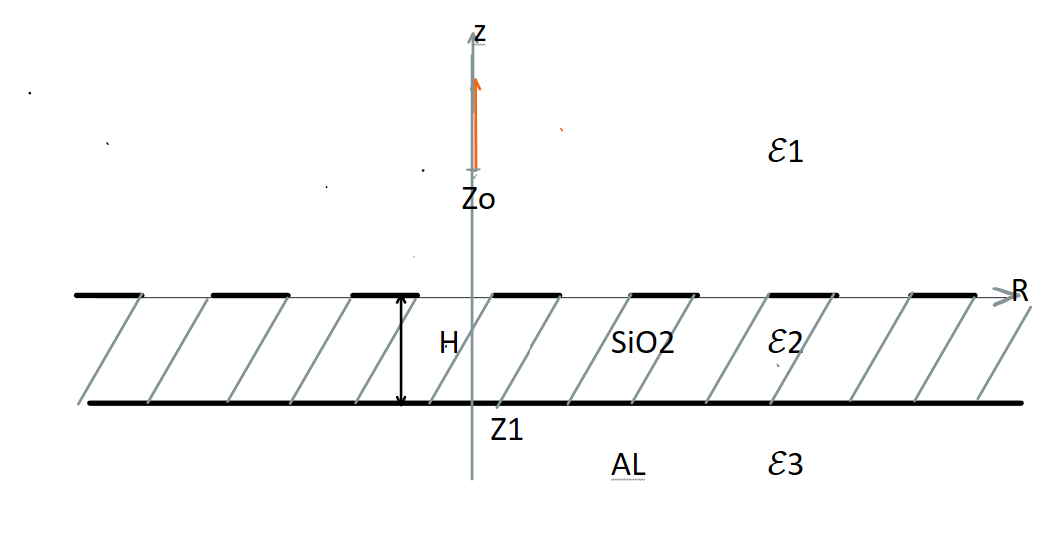
\includegraphics[width=0.5\textwidth]{Рис 1 Вертикальный.PNG} % Вставка изображения. Укажите путь к вашему изображению вместо example-image
		\caption{Плоскослоистая среда с вертикальным дипольным источником} % Подпись к рисунку
		\label{fig:example} % Метка для ссылки на рисунок
	\end{figure}
	
	Для данной задачи запишем систему уравнений Максвелла:
	
	
	\begin{equation}
		\begin{cases} rot \vec{H} = -i \omega \varepsilon \vec{E} + j_{ст} \\ rot \vec{E} = iw\mu \vec{H} \end{cases}
	\end{equation}
	
	Где $\varepsilon(z) = \varepsilon_{re}(z) + i \varepsilon_{im}(z)$ - комплексная диэлектрическая проницаемость.
	
	А магнитная проницаемость среды $\mu$ равна магнитной проницаемости вакуума $\mu_0$
	
	На границе $z = z_1$ выполняются условия непрерывности касательных компонент полей-
	
	\begin{equation}
		\begin{cases} [\vec{n} \times \vec{E} ]_S = 0, \\ [\vec{n} \times \vec{H}]_S = 0 \end{cases}
	\end{equation}
	
	где $[\cdot]$ - разность предельных значений на границе. 
	
	\newpage
	
	Но на границе с графеновым слоем имеется разрыв касательной компоненты H:
	
	\begin{equation*}
		\tag{2.1}
		\begin{cases} 
			[\vec{n} \times \vec{E} ]_S = 0, \\ 
			[\vec{n} \times \vec{H}]_S = \sigma_G E_{\tau} 
		\end{cases}
	\end{equation*}
	
	Комплексная проводимость графена $\sigma_G$ в работах [,], описывается следующей формулой:
	
	$$\sigma_G = \sigma_1 + \sigma_2 * |E_{\tau}^2|$$
	
	далее будет расматриваться микрометровый диапозон источника, при котором $\sigma_2 = 0$
	
	
	Введем 2 векторных потенциала - $A$ и $a$ с калибровками Лоренца:
	
	
	
	\begin{equation}
		\begin{cases}
			\vec{H} = \frac{k^2_{1, 2}a}{\mu_0} + \frac{grad div \vec{a}}{\mu_0} + \frac{rot \vec{A}}{\mu_0} \\
			\vec{E} = i \omega rot \vec{a} +  i \omega \vec{A} + grad(\frac{i \omega}{k^2_{1, 2}} div \vec{A}) 
		\end{cases}
	\end{equation}
	
	\begin{equation*}
		\begin{cases}
			\vec{H^{**}_{1, 2}} = \frac{rot \vec{A}}{\mu_0} \\
			\vec{E^{**}_{1, 2}} = i \omega \vec{A} + grad(\frac{i \omega}{k^2_{1, 2}} div \vec{A}) \\
		\end{cases}
	\end{equation*}
	
	Граничные условия (2.1) можно переписать в виде:
	
	\begin{equation*}
		\tag{2.2}
		\begin{cases}
			[E_x] = 0 \\
			[E_y] = 0 \\
			[H_x] = \sigma_G E_{x_1} \\
			[H_y] = \sigma_G E_{y_1}
			
		\end{cases}
	\end{equation*}
	
	\subsection{Вертикальный диполь}
	
	
	Так как в работе рассматривается вертикальный диполь, то $A, a$ принимают вид:
	
	\begin{equation*}
		A = 
		\begin{pmatrix}
			0 \\ 0 \\ A_z \\
		\end{pmatrix}
		a = 
		\begin{pmatrix}
			0 \\ 0 \\ a_z
		\end{pmatrix}
	\end{equation*}
	
	\newpage
	
	
	
	
	
	так как 
	
	\begin{equation}
		\begin{aligned}
			H_x = \frac{1}{\mu_0} (\frac{\partial ^ 2 a_z}{\partial x \partial z} + \frac{\partial A_z}{\partial y}) \\
			H_y = \frac{1}{\mu_0} (\frac{\partial ^ 2 a_z}{\partial y \partial z} - \frac{\partial A_z}{\partial x}) \\
			E_x = i \omega \delta (\frac{1}{k_1^2} \frac{\partial^2 A_{z_1}}{\partial y \partial z} - \frac{\partial a_{z_1}}{\partial x}) \\			
			E_y = i \omega \delta (\frac{1}{k_1^2} \frac{\partial^2 A_{z_1}}{\partial x \partial z} + \frac{\partial a_{z_1}}{\partial y})
		\end{aligned}
	\end{equation}
	
	то при $z \neq z_0$ $A_z$ и $a_z$ удовлетворяют: 
	
	\begin{equation}
		\begin{aligned}
			\Delta A_z + k^2 A_z = 0 \\
			\Delta a_z + k^2 a_z = 0
		\end{aligned}
	\end{equation}
	
	при приближении к источнику должно выполняться:
	
	\begin{equation}
		A_z \rightarrow \frac{M}{4 \pi} \frac{\exp{i k_1 R}}{R} 
	\end{equation}
	
	где, $R = \sqrt{x^2 + y^2 + {(z - z_0)} ^ 2}$.
	
	при $R \rightarrow \infty$ выполняются
	
	\begin{equation}
		\begin{cases}
			A_z = O_{R \rightarrow \infty}(\frac{1}{R}) \\
			\frac{\partial A_z}{\partial R} + i A_z k = o_{R \rightarrow \infty}(\frac{1}{R})
		\end{cases}
	\end{equation}
	
	Подставив (3) в (2.2) получим при $z = 0$:
	
	\begin{equation}
		\begin{cases}
			\frac{1}{k_1^2} \frac{\partial A_{z_1}}{\partial z} = \frac{1}{k_2^2} \frac{\partial A_{z_2}}{\partial z} \\
			
			a_{z_1} = a_{z_2} \\
			
			-\frac{\partial A_{z_2}}{\partial x} + \frac{\partial^2 a_{z_2}}{\partial y \partial z} + \frac{\partial A_{z_1}}{\partial x} - \frac{\partial^2 a_{z_1}}{\partial y \partial z} = i \sigma_G \delta (\frac{1}{k_1^2} \frac{\partial^2 A_{z_1}}{\partial y \partial z} - \frac{\partial a_{z_1}}{\partial x}) \\
			
			\frac{\partial A_{z_2}}{\partial y} + \frac{\partial^2 a_{z_2}}{\partial x \partial z} - \frac{\partial A_{z_1}}{\partial y} - \frac{\partial^2 a_{z_1}}{\partial x \partial z} = i \omega \sigma_G (\frac{1}{k_1^2} \frac{\partial^2 A_{z_1}}{\partial x \partial z} + \frac{\partial a_{z_1}}{\partial y})
			
			
		\end{cases}
	\end{equation}
	
	при $z = z_1$:
	
	\begin{equation}
		\begin{cases}
			\frac{1}{k_1^2} \frac{\partial A_{z_1}}{\partial z} = \frac{1}{k_2^2} \frac{\partial A_{z_2}}{\partial z} \\
			
			a_{z_1} = a_{z_2} \\
			
			-\frac{\partial A_{z_2}}{\partial x} + \frac{\partial^2 a_{z_2}}{\partial y \partial z} + \frac{\partial A_{z_1}}{\partial x} - \frac{\partial^2 a_{z_1}}{\partial y \partial z} = 0 \\
			
			\frac{\partial A_{z_2}}{\partial y} + \frac{\partial^2 a_{z_2}}{\partial x \partial z} - \frac{\partial A_{z_1}}{\partial y} - \frac{\partial^2 a_{z_1}}{\partial x \partial z} = 0
			
			
		\end{cases}
	\end{equation}
	
	Будем искать решение в виде преобразований Ханкеля (аналогично случаю без графена)
	
	\begin{equation}
		\begin{aligned}
			a_z = \frac{I \mu_0 }{4 \pi} \int_0^{\infty} X J_0(mz)dm \\
			A_z = \frac{I \mu_0 }{4 \pi} \int_0^{\infty} V J_0(mz)dm
		\end{aligned}
	\end{equation}
	
	X и V будем искать в виде:
	\begin{equation}
		\begin{cases}
			X_1 = d_1 e^{-n_1 z}, z > 0 \\
			X_2 = d_2 e^{-n_2 z} + c_2 e^{n_2 z}, 0 < z < z_1 = H \\
			X_3 = c_3 e^{-n_3 z}, z < H
			
		\end{cases}		
	\end{equation}
	
	\begin{equation}
		\begin{cases}
			\tilde{V_1} = \tilda{\beta_1^} e^{-n_1 z}, z > z_0 \\
			V_1 = \beta_1 e^{-n_1 z} + \gamma_1 e^{n_1 z}, 0 < z < z_0 \\
			V_2 = \beta_2 e^{-n_2 z} + \gamma_2 e^{n_2 z}, z_1 < z < 0 \\
			V_3 = \gamma_3 e^{n_3 z}, z < z_1
		\end{cases}
	\end{equation}
	
	Через $z = z_0$ проведена фиктивная граница, чтобы в точке $z = z_0$ где находится источник получить необходимую особенность для компоненты $A_z$
	векторного потенциала.
	
	
	тогда $X$ и $V$ удовлетворяют
	
	\begin{equation}
		\begin{aligned}
			\frac{\partial^2 X}{\partial z^2} - n_{1, 2}^2 X = 0 \\
			\frac{\partial^2 V}{\partial z^2} - n_{1, 2}^2 V = 0 \\
		\end{aligned}
	\end{equation}
	
	где $n_{1, 2}^2 = m^2 - k_{1, 2}^2$, $Re (n) > 0$
	
	
	для $X$ и $V$ получим в $z = 0$:
	
	\begin{equation}
		\begin{aligned}
			& \frac{1}{k_1^2} \frac{\partial V_1}{\partial z} = \frac{1}{k_1^2} \frac{\partial V_2}{\partial z} \\
			&X_1 = X_2 \\
			& V_2 - V_1 = i \omega \sigma_G X_2 \\
			&\frac{\partial X_2}{\partial z} - \frac{\partial X_1}{\partial z} = -i \omega \sigma_G \frac{1}{k_2^2} \frac{\partial V_2}{\partial z} \\ 
		\end{aligned}
	\end{equation}
	
	для $X$ и $V$ получим в $z = z_1$:
	
	\begin{equation}
		\begin{aligned}
			& \frac{1}{k_1^2} \frac{\partial V_1}{\partial z} = \frac{1}{k_1^2} \frac{\partial V_2}{\partial z} \\
			&X_1 = X_2 \\
			& V_2 - V_1 = 0 \\
			&\frac{\partial X_2}{\partial z} - \frac{\partial X_1}{\partial z} = 0 \\ 
		\end{aligned}
	\end{equation}
	\newpage
	в $z = z_0$
	
	
	\begin{equation}
		\begin{aligned}
			&\frac{\partial \tilde{V_1}}{\partial z} - \frac{\partial V_1}{\partial z} = 2 \\
			&\tilde{V_1} = V_1 \\
		\end{aligned}
	\end{equation}
	
	
	Из (14-16) получим систему линейных адгебраических уравнений. После решения этой систему линейных адгебраических уравнений получим:
	
	\begin{equation}
		\begin{aligned}
			&d_1 = - \frac{2 Q \gamma_1}{1 - N - Qi\omega \delta} \\
			&c_2 = \frac{d_1}{1 + L} \\
			&d_2 = \frac{l d_1}{1 + L} \\
			&d_3 = \frac{d_1}{1 + L} e^{n_3 z_1}(l e^{n_2 z_1} + e^{-n_2 z_1}) \\
			&\tilde{\beta_1} = \beta_1 + \gamma_1 e^{-2 n_1 z_0} \\
			&\gamma_1 = -\frac{k_1^2}{n_1} e^{n_1 z_1} \\
			&\beta_1 = \frac{-\gamma_1(1 + N) + i \omega \delta d_1}{1 - N} \\
			&\beta_2 = \frac{\beta_1 + \gamma_1 - i \omega \delta d_1}{1 + M} \\
			&\gamma_2 = \beta_2 e^{2 n_2 z_1} \frac{q}{p} \\
			&\gamma_3 = \beta_2 e^{n_3 z_1}e^{n_2 z_1}(1 + \frac{q}{p})
			
			
			
		\end{aligned}
		
	\end{equation}
	
	где введены следующие обохначения:
	\begin{equation}
		\begin{aligned}
			&q = \frac{n_2}{k_2^2} - \frac{n_3}{k_3^2} \\
			&p = \frac{n_2}{k_2^2} + \frac{n_3}{k_3^2} \\
			&R = L = \frac{n_2 - n_3}{n_2 + n_3} e^{-2n_2 z_1} \\
			&r = M = e^{-2 n_2 z_1}\frac{q}{p} \\
			&N = \frac{1 + M}{1 - M}\frac{k_2^2 n_1}{k_1^2 n_2} \\
			&Q = \frac{i \omega \delta}{k_1^2} (1 - \frac{n_2}{n_1}\frac{1 - L}{1 + L})
		\end{aligned}
	\end{equation}
	
	$\tilde{V_1} и V_1$ при $z > 0$ можно объеденить в один случай $V_1$ и тогда $V_1$ принимает виды
	
	\begin{equation}
		\begin{aligned}
			&V = 2 \frac{\varepsilon_2 (R + 1) (\eta_2 (1 - r) + \eta_1(1 + r)) - \mu \sigma_G^2 \eta_2 (R - 1) (r + 1)}{(\varepsilon_2 \eta_1 (R + 1) - \varepsilon_1 \eta_2 (R - 1))(\eta_2 (1 - r) + \eta_1(1 + r)) - \mu \sigma_G^2 \eta_1 \eta_2 (R - 1)(r + 1)} \\
			&\frac{e^{-\eta_1(z + z_0)}}{\eta_1} + \frac{e^{-\eta_1(z + z_0)}}{\eta_1}
		\end{aligned}
		
	\end{equation}
	
	А $X$ можно представить в виде:
	
	
	
	\begin{equation}
		\begin{aligned}
			&\frac{\eta_2(R - 1) (R + 1)}{(\varepsilon_2 \eta_1 (R + 1) - \varepsilon_1 \eta_2 (R - 1)) 
				(\eta_2 (1 - r) + \eta_1 (1 + r)) - \mu \sigma_G^2 \eta_1 \eta_2 (R - 1) (1  + r)} \cdot 
			\frac{2i \sigma_G}{\omega} \\
			& \frac{e^{-\eta_1(z + z_0)}}{\eta_1} + \frac{e^{-\eta_1(z + z_0)}}{\eta_1}
		\end{aligned}
		
	\end{equation}
	
	\newpage
	
	Компоненты электромагнитного поля вертикального диполя в слоистой среде
	в цилиндрической системе координат вычисляется по следующим формулам
	\begin{equation*}
		\begin{aligned}
			a_z = \frac{\mu_0 }{4 \pi} \int_0^{\infty} X(\lambda, z, z_0) J_0(\lambda \rho)\lambda d \lambda \\
			A_z = \frac{\mu_0 }{4 \pi} \int_0^{\infty} V(\lambda, z, z_0) J_0(\lambda \rho) \lambda d \lambda
		\end{aligned}
	\end{equation*}
	
	Так как коефициенты в X, V зависят исключительно от $\lambda$ то можно вычислить $\frac{\partial^2 A_z}{\partial z^2}, \frac{\partial_2 A_z}{\partial z \partial \rho}, \frac{\partial A_z}{\partial \rho}, \frac{\partial^2 a_z}{\partial z^2}, \frac{\partial_2 a_z}{\partial z \partial \rho}, \frac{\partial a_z}{\partial \rho}, $
	
	Сравним компонеты поля в случае с наличием графена и его отсутствием:
	
	\begin{equation}
		\begin{array}{c|c}
			\begin{aligned}
				\begin{cases}
					$$E_{\rho} = -\frac{1}{i \omega \varepsilon \mu} \frac{\partial^2 A_z}{\partial z \partial \rho}$$ \\
					$$E_{\phi} = - i \omega \frac{\partial a_z}{\partial \rho}$$ \\
					$$E_z = i \omega A_z - \frac{1}{i \omega \varepsilon \mu} \frac{\partial^2 A_z}{\partial z^2}$$ \\
					$$H_{\rho} = \frac{1}{\mu} \frac{\partial^2 a_z}{\partial \rho \partial z}$$ \\
					$$H_{\phi} = \frac{1}{\mu} \frac{\partial A_z}{\partial \rho}$$ \\
					$$H_{z} = \frac{1}{\mu}(k^2 a_z +  \frac{\partial^2 a_z}{\partial z \partial z})$$ \\
					
					
					
				\end{cases}
			\end{aligned}
			&
			\begin{aligned}
				\begin{cases}
					$$E_{\rho} = -\frac{1}{i \omega \varepsilon \mu} \frac{\partial^2 A_z}{\partial z \partial \rho}$$ \\
					$$E_{\phi} = 0$$ \\
					$$E_z = i \omega A_z - \frac{1}{i \omega \varepsilon \mu} \frac{\partial^2 A_z}{\partial z^2}$$ \\
					$$H_{\rho} = 0$$ \\
					$$H_{\phi} = \frac{1}{\mu} \frac{\partial A_z}{\partial \rho}$$ \\
					$$H_{z} = 0$$ \\
					
					
					
				\end{cases}
			\end{aligned}
			
		\end{array}
	\end{equation}
	
	Можно заметить что при отсутсвии графена $\sigma_G = 0$ и $a_z$ вырождается в 0 и полученные выражения сводятся к выражениям без графена, что потдтвержает корректность формул.
	
	\newpage
	
	
	
	
	\section{Выводы}
	
	В результате работы были получены следующие результаты:
	\begin{itemize}
		\item Задача вычисления электромагнитного поля вертикального электрического диполя, который находится в верхнем полупространстве плоскослоистой среды, содержащей слой графена, была сведена к задаче вычисления двух векторных потенциалов, которые обеспечивают выполнение условий для тангенциальных компонент электромагнитного поля на границе с графеном.
		\item	Получены формулы для вычисления компонент электромагнитного поля вертикального электрического диполя с использованием векторных потенциалов.
		\item 	Создана программа для вычисления компонент электромагнитного поля вертикального электрического диполя для модели среды, в которой слой графена находится на границе верхнего полупространства и диэлектрического слоя, который лежит на проводящем полупространстве. 
		
	\end{itemize}
	
	\newpage 
	
	\section{Литература}
	
	\begin{itemize}
		\item [1] Тихонов А. Н. Самарский А. А. Уравнения математической физики: Учебное пособие - 6е издание Изд-во МГУ 1999. ISBN 5-211-04138-0 
		
		\item [2] Дмитриев В. И. Захаров Е. В. Метод интегральных уравнений в вычислительной электродинамике. МАКС Пресс 2008 - 316с ISBN 978-5-317-02657-8
		
		\item [3] Давыдов В. М. Теория низкочастотных электромагнитных полей в средах с тонкими анизотропными слоями и ее геофизические приложения. Новосибирск 1971.
		
		\item [4] S. A. Mikhailov
		Non-linear electromagnetic response of graphene
		Institute for Theoretical Physics II, University of Augsburg, D-86135
		Augsburg, Germany (Dated: February 5, 2008)
		
		\item [5] Linear and Nonlinear Optical Properties of Graphene: A Review
		Vipin Kumar Journal of Electronic Materials (2021) 50:3773–3799
		
		\item [6] Линейные и нелинейно-оптические свойства графена: обзор
		Випин Кумар - Журнал электронных материалов, 2021 - Springer
		
		\item [7] S. A. Mikhailov
		Institute for Theoretical Physics II, University of Augsburg, D-86135 Augsburg, Germany
		(Dated: October 22, 2018)
		
		\item [8] A. K. Geim and K. S. Novoselov, Nature Materials 6, 183 (2007).
		
		\item [9] Электромагнитное поле диполя в анизотропной среде
		© А.О. Савченко,1 О.Я. Савченко Журнал технической физики, 2005, том 75, вып. 1
		
		\item  [10] Dmitriev V. I., Silkin A. N., Farzan R. Tensor green function for the system of maxwell’s equations in a layered medium // Computational Mathematics and Modeling. — 2002. — Vol. 13, no. 2. — P. 107–118. 
		
		\item [11] Вестник СибГУТИ. 2016. № 2
		УДК 621.396.67
		Тензорные функции Грина
		для расчета электромагнитных полей 
		от слоистых сферических структур
		Б. А. Панченко, Д. В. Денисов, А. М. Муcин, И. О. Скумотенко
		
		\item [12] G. W. Hanson, Dyadic Green’s functions and guided surface
		waves for a surface conductivity model of graphene, Journal of
		Applied Physics, vol. 103, no. 6, p. 064302, 2008, doi:
		https://doi.org/10.1063/1.2891452
		
		\item [13] Дмитриев В.И. Общий метод расчета электромагнитного поля
		в слоистой среде. – В сб. Вычислительные методы и
		программирование, вып.10. Изд. Московского университета,
		1968, 316 стр. 55- 65.
		
		\item [14] О. А. Голованов, Г. С. Макеева, В. В. Вареница. Проводимость
		графена в терагерцовом и инфракрасном диапазонах частот. –
		Надежность и качество сложных систем, 2014, № 4 (8), с.
		26–33.
		
		\item  [15] RefractiveIndex.INFO - Refractive index database.
		\item 16 Ю. Г. Смирновб С.В Тихов. Расспостранение электромагнитных TE- и TM- волн в плоском волноводе, покрытом графеном, с учетом нелинейности. - Физика волновых процессов и радиотехнические схемы, 2023. Т. 26, номер 4. с 
		68-77
		
		
		
		\item [16] Кулакова И. Ию Лисичкин Г. В. Перспективы применения графеновых наноматериалов: 
		сорбенты, мембраны, газовые сенсоры (обзор). - Журнал прикладной химии, 2021, том 94, вып.9, с 1090 - 1103.
		
		
		
		\item [17] Vipin Kumar. Linear and Nonlinear Optical Properties of Graphene:
		A Review. Journal of Electronic Materials (2021) 50:3773–3799 \newline
		https://doi.org/10.1007/s11664-021-08904-w 
	\end{itemize}
	
	
	
\end{document}